\chapter{Two Processors}
\label{chap:p2}

\section{Another recursion describing optimal expected run time}
\label{sec:p2-simple-method-for-runtime}

If one considers the problem of scheduling an intree onto two processors, it becomes clear that HLF is optimal (\todo{Proof.}). Moreover, we can conclude that we can compute the optimal expected finish time in polynomial time.

This section shows how the original problem of an intree DAG can be mapped onto another, more compact structure.

If we consider the trees in figure \ref{fig:p2-four-intrees-with-same-profile-6-3-1}, we can compute that for two processors HLF always yields an expected run time of $\frac{49}{8}$ for each of them, which is optimal:

\begin{figure}[ht]
  \centering
  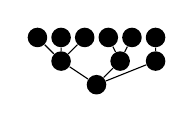
\begin{tikzpicture}[scale=.2]
\node[circle, scale=0.75, fill] (tid0) at (4.5,1.5){};
\node[circle, scale=0.75, fill] (tid1) at (2.25,3){};
\node[circle, scale=0.75, fill] (tid4) at (0.75,4.5){};
\node[circle, scale=0.75, fill] (tid5) at (2.25,4.5){};
\node[circle, scale=0.75, fill] (tid6) at (3.75,4.5){};
\draw[](tid1) -- (tid4);
\draw[](tid1) -- (tid5);
\draw[](tid1) -- (tid6);
\node[circle, scale=0.75, fill] (tid2) at (6,3){};
\node[circle, scale=0.75, fill] (tid7) at (5.25,4.5){};
\node[circle, scale=0.75, fill] (tid8) at (6.75,4.5){};
\draw[](tid2) -- (tid7);
\draw[](tid2) -- (tid8);
\node[circle, scale=0.75, fill] (tid3) at (8.25,3){};
\node[circle, scale=0.75, fill] (tid9) at (8.25,4.5){};
\draw[](tid3) -- (tid9);
\draw[](tid0) -- (tid1);
\draw[](tid0) -- (tid2);
\draw[](tid0) -- (tid3);
\end{tikzpicture}
%%% Local Variables:
%%% TeX-master: "thesis/thesis.tex"
%%% End: \hspace{0.5cm}
  \input{p2/000111122_profile}\hspace{0.5cm}
  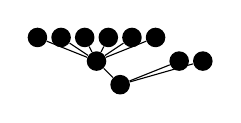
\begin{tikzpicture}[scale=.2]
\node[circle, scale=0.75, fill] (tid0) at (6,1.5){};
\node[circle, scale=0.75, fill] (tid1) at (4.5,3){};
\node[circle, scale=0.75, fill] (tid4) at (0.75,4.5){};
\node[circle, scale=0.75, fill] (tid5) at (2.25,4.5){};
\node[circle, scale=0.75, fill] (tid6) at (3.75,4.5){};
\node[circle, scale=0.75, fill] (tid7) at (5.25,4.5){};
\node[circle, scale=0.75, fill] (tid8) at (6.75,4.5){};
\node[circle, scale=0.75, fill] (tid9) at (8.25,4.5){};
\draw[](tid1) -- (tid4);
\draw[](tid1) -- (tid5);
\draw[](tid1) -- (tid6);
\draw[](tid1) -- (tid7);
\draw[](tid1) -- (tid8);
\draw[](tid1) -- (tid9);
\node[circle, scale=0.75, fill] (tid2) at (9.75,3){};
\node[circle, scale=0.75, fill] (tid3) at (11.25,3){};
\draw[](tid0) -- (tid1);
\draw[](tid0) -- (tid2);
\draw[](tid0) -- (tid3);
\end{tikzpicture}
%%% Local Variables:
%%% TeX-master: "thesis/thesis.tex"
%%% End: \hspace{0.5cm}
  \begin{tikzpicture}[scale=.2]
\node[circle, scale=0.75, fill] (tid0) at (5.25,1.5){};
\node[circle, scale=0.75, fill] (tid1) at (2.25,3){};
\node[circle, scale=0.75, fill, task_scheduled] (tid4) at (0.75,4.5){};
\node[circle, scale=0.75, fill] (tid5) at (2.25,4.5){};
\node[circle, scale=0.75, fill] (tid6) at (3.75,4.5){};
\draw[](tid1) -- (tid4);
\draw[](tid1) -- (tid5);
\draw[](tid1) -- (tid6);
\node[circle, scale=0.75, fill] (tid2) at (6.75,3){};
\node[circle, scale=0.75, fill, task_scheduled] (tid7) at (5.25,4.5){};
\node[circle, scale=0.75, fill] (tid8) at (6.75,4.5){};
\node[circle, scale=0.75, fill] (tid9) at (8.25,4.5){};
\draw[](tid2) -- (tid7);
\draw[](tid2) -- (tid8);
\draw[](tid2) -- (tid9);
\node[circle, scale=0.75, fill] (tid3) at (9.75,3){};
\draw[](tid0) -- (tid1);
\draw[](tid0) -- (tid2);
\draw[](tid0) -- (tid3);
\end{tikzpicture}
%%% Local Variables:
%%% TeX-master: "thesis/thesis.tex"
%%% End: 
  \caption{Four intrees with the same profile ($\profile{6,3,1}$). All of them have expected run time of $49/8$ if scheduled with HLF on two processors.}
  \label{fig:p2-four-intrees-with-same-profile-6-3-1}
\end{figure}

The intrees in figure \ref{fig:p2-four-intrees-with-same-profile-6-3-1} have the following in common: At each level, they have the same amount of tasks (six tasks at the topmost level, three in the middle one and one at the bottom level).

We can use the number of tasks per level as a (non-bijective) ``encoding'' of intrees. For now, we call this encoding a \emph{profile} of the intree. The above intrees would all be encoded as a profile containing the numbers 6, 3 and 1 in that order. We denote the profile by $\llbracket 6, 3, 1 \rrbracket$.

Note that not all sequences of numbers can be used as profiles. In particular, the last number in a profile is (w.l.o.g.) 1 (since we have only one task as the root of the tree). Moreover, it can not be the case that there is a zero in a profile (since this would imply that there is \emph{no task} on one specific level in the intree).

\newcommand{\profile}[1]{\llbracket #1 \rrbracket}

Moreover, for two processors and HLF-scheduling, we can easily conclude the successors of a profile. Let us consider an example here: If we have the profile $\llbracket 5,4,2,1 \rrbracket$, then 2 of the 5 topmost tasks have to be scheduled. If one of these tasks is finished, we reach $\profile{4,4,2,1}$.

Another interesting case is $\profile{1,5,2,1}$, where the (single) topmost task and one of the 5 tasks on the second level are scheduled. If the topmost task is finished (which happens with probability $\frac{1}{2}$), we reach $\profile{5,2,1}$. If the scheduled task on the second level finishes first, we reach $\profile{1,4,2,1}$.

We now use the profile notation to denote the expected run time (i.e. we say $\profile{6,3,1} = \frac{49}{8}$ --- see image above).

Exploiting this notation, we can define the following recursive formula that can be used to compute the optimal expected run time:

\begin{equation}
  \label{eq:p2-profile-optimal-exp-run-time}
  \profile{n_1, \dots, n_r} =
  \begin{cases}
    r, & \text{ if } n_1 = n_2 = \dots = n_r = 1 \\
    \frac{n_1-1}{2} + \profile{1, n_2, n_3, \dots, n_r} , & \text{ if } n_r\geq 2 \\
    \frac{1}{2} + \frac{1}{2} \cdot \left( \profile{n_2, \dots, n_r} + SUC(\profile{n_1,\dots,n_r}) \right) ,& \text{ otherwise }
  \end{cases},
\end{equation}
where $SUC(\profile{n_1,\dots,n_r}) = \profile{n_1, n_2, n_3,\dots,n_{j-1},n_j-1,n_{j+1},\dots,n_r}$ such that $j$ is the minimum index such that $n_j>1$.

We can simplify equation (\ref{eq:p2-profile-optimal-exp-run-time}) to the following:

\begin{equation}
  \label{eq:p2-profile-optimal-exp-run-time-def-simplified}
  \profile{n_1, \dots, n_r} =
  \begin{cases}
    r, & \text{ if } n_1 = n_2 = \dots = n_r = 1 \\
    \frac{n_1}{2} + \frac{1}{2} \cdot \left( \profile{n_2, \dots, n_r} + SUC(\profile{1,n_2,\dots,n_r}) \right) ,& \text{ otherwise }
  \end{cases},
\end{equation}
with $SUC$ as defined before.

Unfortunately, this recurrence relation does not make the original problem much more easy. However, we were able to deduce the following conjecture.

\begin{conjecture}
  Let $\profile{n_1,n_2,\dots,n_r}$ be a profile where 
  $\left|\left\{ i \in \left\{ 2,3,\dots,r \right\} \mid n_i > 1 \right\}\right| \leq 1$ 
  (i.e. all but at most two profile entries -- including the first one -- are 1).
  Then we can compute 
  \begin{equation*}
    \profile{n_1,n_2,\dots,n_r} = \sum_{i=1}^r \left( \frac{A_i(n_i)}{2^{n_i+i-2}} \right),
  \end{equation*}
  where $A_i$ is inductively defined as follows:
  \begin{align*}
    A_0(n) & = (n+1) \cdot 2^n \\
    A_{i+1}(n) & = \sum_{k=1}^n A_{i}(k)
  \end{align*}
\end{conjecture}

Note that there are closed expressions for $A_i(n)$ for a fixed $i$. However, these formulae are quite complex and do not contribute to clarity, which is why we omit them here.

We examined this conjecture, but we were not able to deduce a more general formula that holds if more entries in the profile differ from 1.

%%% Local Variables:
%%% TeX-master: "../thesis.tex"
%%% End: 